\clearpage

\section{Score-based models}\label{sec:scorebased}\index{score-based models}

\begin{notebox}
\textbf{Paper: } \fullcite{song_generative_2020}
\vspace{5pt}

\href{https://papers.nips.cc/paper/2019/file/3001ef257407d5a371a96dcd947c7d93-Reviews.html}{reviews}
\hspace{1cm}
\href{https://github.com/yang-song/score_sde_pytorch}{code}
\hspace{1cm}
\href{run:/home/magda/Dropbox/Zot/Song_Ermon_2020_Generative Modeling by Estimating Gradients of the Data Distribution.pdf}{Local pdf}
\vspace{3pt}

Read with Simon\index{Simon} on 9/2/2022
\hfill Notes taken: 14/2/2022 \index{February 2022}
\end{notebox}

\begin{notebox}[colback=red!5]
\tldr 
Generative model where data are generated through Langevin dynamics \parencite{welling_bayesian_2011} using gradients estimated through score matching \parencite{hyvarinen_estimation_2005}.
They perturb the data with small Gaussian noise to ensure the data don't lie on a low dimensional manifold within the original feature space which would make the gradients ill-defined. They also propose to anneal the Langevin dynamics sampling process with gradually decreasing noise levels.
\end{notebox}

\begin{notebox}[colback=yellow!5]
\textbf{Notes:} 
\begin{itemize}[nosep]
\item Mixing a lot of things together into something that in the end works
\item A bit of archeology to dig up score mathchin and Langevin dynamics sampling
\item The random projections idea is here nonsensical I think, it is a different setup. They put it just to increase citation score? ;)
\item The perturbation story holds in retrospect but I wonder how did they come up with it in the first place.
\end{itemize}
\end{notebox}



The model is based on estimating the (Stein) \emph{\textbf{score\index{index} that is the gradient of the log data density with respect to the data $\nabla_{\rvx} \log p(\rvx)$}} (though standard score function in statistics is the gradient with respect to the parameters of the distribution at a fixed data point - this is acknowledged in the original [33] paper of Jordan's group but not in this paper).

The score network $s_\theta: R^D \to R^D$ shall be trained to estimate the score without estimating the data likelihood $p(\rvx)$ first. Once trained, it can be used within Langevin dynamics sampling to generate new data examples.

The \textbf{score matching}\index{score matching} objective is the minimization of $0.5 \E_{p_{data}} \Vert s_{\theta}(\rvx) - \nabla_{\rvx} \log p(\rvx) \Vert_2^2$ which has been show (in \cite{hyvarinen_estimation_2005} to be equivalent to the minimization of
\begin{align*}
\E_{p_{data}}(\rvx) \left[ tr(\nabla_\rvx s_\theta(\rvx)) + \frac{1}{2} \Vert s_\theta(\rvx) \Vert_2^2 \right]
\end{align*}
This is important cause it removes the unknown data density $p(\rvx)$ from the loss. The problem is, however, that it does not scale to high dimensions because of the need to get the trace of the jacobian. \note{Because of the jacobian?}

Instead, they propose to use the \textbf{denoising score matching}\index{denoising score matching}
\begin{align*}
\frac{1}{2} \E_{q_\sigma(\widetilde\rvx|\rvx)} \left[ \Vert s_{\theta}(\widetilde\rvx) - \nabla_{\widetilde\rvx} \log q_\sigma(\widetilde\rvx|\rvx) \Vert_2^2 \right]
\end{align*}
which is shown in \cite{vincent_connection_2011} to be equivalent to score matching with the marginal
$q_\sigma(\widetilde\rvx) = \int q_\sigma(\widetilde\rvx | \rvx) p_{data}(\rvx) d\rvx$ \note{Not very intuitive but I trust the proof}. In turn this would also be equivalent to score matching with the original data density $p_{data}$ if the noise is very little so that $q_\sigma(\rvx) \approx p_{data}(\rvx)$.

Finally, they claim by the use of \textbf{random projections}\index{random projections} they can reduce the complexity of the trace jacobian calculation recognized above.
\begin{align*}
\E_{p_v} \E_{p_{data}} \left[ \rvv^T \nabla_\rvx s_{\theta}(\rvx) \rvv - \frac{1}{2} \Vert s_{\theta}(\rvx) \Vert_2^2 \right]
\end{align*}
\note{I don't see how this helps cause you still need to get the jacobian. Hm ... }

Once they have trained the score estimator $s_{\theta}(\rvx) \approx \nabla_{\rvx} \log p(\rvx)$ they can use \textbf{Langevin dynamics}\index{Langevin dynamics} as explained in \cite{welling_bayesian_2011} to sample examples
\begin{align*}
\hat\rvx_t = \hat\rvx_{t-1} + \frac{\epsilon}{2} s_{\theta}(\hat\rvx_{t-1}) + \sqrt{\epsilon} \rvz_t \enspace , 
\end{align*}
where $\rvz_t \sim \mathcal{N}(0, \mI)$ is the noise, $\hat\rvx_0$ sampled from a prior $\pi(\rvx)$ and step size $\epsilon > 0$.
When $\epsilon \to 0$ and $T \to \infty$ then $\hat\rvx_T$ has the same distribution as the desired $p(\rvx)$. 
\begin{notebox}
This is a kind of gradient ascent with noise. I can see that we gradually move the samples to a higher density region and adding a little bit of noise while doing it. How come that in infinity with decreasing noise all the $\hat\rvx_T$ do not end in the mode of the distribution? I guess \cite{welling_bayesian_2011} has the answer :).
\end{notebox}

They next claim that because the data may reside on a \emph{low dimensional manifold}, the gradient of the density in the original feature space may be ill-defined.
Furthermore, the model struggles at \emph{low density regions}. It is difficult to estimate the score correctly in these regions due to undersampling. Similarly, Langevin dynamics cannot balance mixtures of distributions correctly. 
They solve these by perturbing the data with various levels of noise $\sigma$ (a decreasing schedule) and then estimating the corresponding scores by training a score network conditioned on the noise level $s_{\theta}(\rvx, \sigma)$.
This naturally leads back to the denoising score matching version of the loss optimization which moreover with Gaussian perturbations $q_\sigma(\widetilde\rvx|\rvx) \sim \mathcal{N}(\rvx, \sigma\mI)$ nicely simplifies to 
\begin{align*}
l(\theta, \sigma) & = \frac{1}{2} \E_{p_{data}(\rvx)} \E_{q_\sigma(\widetilde\rvx|\rvx)} \left[ \Vert s_{\theta}(\widetilde\rvx) - \frac{\tilde\rvx - \rvx}{\sigma^2} \Vert_2^2 \right] \\
\Ls(\theta) & = \frac{1}{L}\sum_i^L \lambda(\sigma_i) l(\theta, \sigma_i)
\end{align*}
so that the final loss is a weighted average of the noisy score losses. They use trivially $\lambda(\sigma_i) = \sigma_i^2$.
\begin{wrapfigure}{l}{0.5\textwidth}
\centering
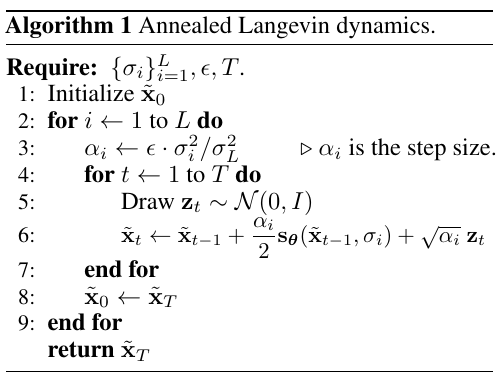
\includegraphics[width=0.5\textwidth]{scoreBased_Algo.png}
\end{wrapfigure}

They then use the noisy estimates of the scores in the Langevin dynamics sampling process - starting from the score estimated from the most noisy data generate a sample through multiple steps of the Langevin dynamics update, then use this sample as the initial point for next iteration of the updates with lower noise. The step size is also gradually decreasing by a fixed schedule according to the noise levels.


Nice experiments showing how the sampled data gradually get cleaner through the annealed Langevin dynamic sampling.


